\chapter{Theory} 
\label{Theory}
\label{theory}

All particles and their interactions at short distances are described by a quantum field theory known as the Standard Model. In the Standard Model there are two fundamental divisions of particles: matter particles (Section~\ref{matter}) and particles which facilitate interactions between the matter particles (Section~\ref{interaction}). The heaviest matter particle in the Standard Model is the top quark and its properties and production via the strong interaction are discussed in Section~\ref{topquark}. Finally, Section~\ref{electroweaktopquark}~explains how the top quark is singly produced via an electroweak interaction.


\section{Standard Model: Matter Particles}
\label{matter}

All matter particles in the Standard Model can be categorized either as quarks or leptons. Quarks are spin-$\frac{1}{2}$~particles that are grouped into three generations. Each generation contains two quarks: one with fractional electric charge +$\frac{2}{3}$e (commonly called up type) and one with charge -$\frac{1}{3}$e (commonly called down type). Leptons are also spin-$\frac{1}{2}$~particles that are grouped into three generations. In the lepton generation, one particle has unit charge ($\pm1$e) and the other has no charge and essentially no mass. The lightest particles in both the quark and lepton generations are found in the first generation while the heaviest are found in the third generation. Table ~\ref{fermions} summarizes the spin-$\frac{1}{2}$ matter particles in the Standard Model.

\begin{table}[!h!tbp]
\begin{center}
\caption{Properties of the fundamental spin-$\frac{1}{2}$ fermions in the Standard Model~\cite{Yao:2006px}.}
\begin{tabular}{c|ccc|ccc}
& \multicolumn{3}{c|}{\underline{Quarks}}
& \multicolumn{3}{c}{\underline{Leptons}} \\
Gen.	&	Flavor	&	Charge	&	Mass [MeV]				&	Flavor					&	Charge	&	Mass [MeV]	\\
\hline
I	&	Up (u)		&	+$\frac{2}{3}$e	&	1.5 to 3.0					&	Electron (e)				&	-e		&	0.511	\\
	&	Down (d)		&	-$\frac{1}{3}$e	&	3 to 7					&	(e) neutrino ($\nu_{e}$)	&	0		&	$<$ 2.2 $\times$ $10^{-6}$	\\
\hline
II	&	Charm (c)		&	+$\frac{2}{3}$e	&	1.25 $\times$ $10^{3}$		&	Muon ($\mu$)				&	-e		&	105.7	\\
	&	Strange (s)	&	-$\frac{1}{3}$e	&	80-130					&	($\mu$) neutrino ($\nu_{\mu}$)	&	0		&	$<$ 1.7 $\times$ $10^{-4}$	\\
\hline
III	&	Top (t)		&	+$\frac{2}{3}$e	&	171.4 $\times$ $10^{3}$		&	Tau ($\tau$)				&	-e		&	1777		\\
	&	Bottom (b)		&	-$\frac{1}{3}$e	&	4.7 $\times$ $10^{3}$		&	($\tau$) neutrino ($\nu_{\tau}$)	&	0		&	$<$ 15.5	\\
\end{tabular}
\vspace{-0.1 in}
\label{fermions}
\end{center}
\end{table}

\section{Standard Model: Particle Interactions}
\label{interaction}

There are three fundamental interactions described by the Standard Model. The first is the electromagnetic interaction between any objects that carry electric charge such as the electron or proton. The second is the weak interaction which, at low energies, is responsible for nuclear beta decay (e.g. neutron $\rightarrow$ proton + electron + neutrino). The third interaction described by the Standard Model is the strong interaction, which binds protons and neutrons together in the atomic nucleus.

The electromagnetic and weak interactions are unified in the Standard Model in an $SU(2)_{L} \otimes U(1)_{Y}$ gauge theory. This theory predicts four force carriers: two neutral ($B$ and $W^{0}$) and two charged  ($W^{\pm}$). These particles are required to explain neutral and charged current interactions, however the theory does not explain why three of these particles are observed to be massive and one is massless. To allow for massive force carriers, a neutral scalar particle ($\phi=[\phi_{1}~\phi_{2}]^{T}$) is added to the theory, with a potential shown in Fig.~\ref{HiggsPotential}. The addition of this particle and its potential breaks the $SU(2)_{L} \otimes U(1)_{Y}$ gauge symmetry. This new term gives mass to the two charged force carries ($W^{\pm}$) and mixes the two neutral particles such that one acquires mass ($Z^{0}$) and the other remains massless ($\gamma$). While this theory is very elegant, its prediction of a neutral scalar particle has yet to be verified experimentally. The search for this particle, known as the Higgs boson, is one of the foremost challenges in high energy physics.

\begin{figure}[!h!tbp]
\begin{center}
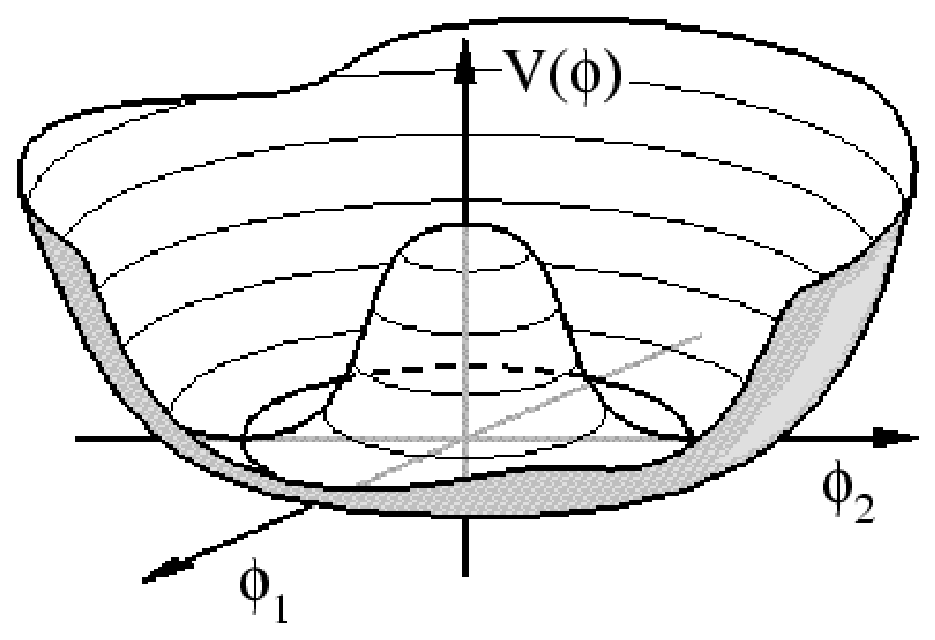
\includegraphics[width=0.50\textwidth]{eps/Theory/HiggsPotential.eps}
\end{center}
\vspace{-0.1in}
\caption{The Higgs "wine-bottle" potential~\cite{higgspotential}.}
\label{HiggsPotential}
\end{figure}

The strong interaction is an SU(3) gauge theory mediated by eight massless gauge bosons called gluons. The gluons interact with any particle that carries color charge, which in the Standard Model are quarks and the gluons themselves. The strong interaction exhibits an interesting property that the strength of the interaction decreases as the energy of the processes increases. Eq.~\ref{alphas}~shows the strong coupling parameter ($\alpha_{S}$) dependence on the energy of the process. 

\begin{equation}
\label{alphas}
\alpha_{S}(E) = \frac{12\pi}{33-2n_{f}\ln\left[\left(\frac{E}{\Lambda}\right)^{2}\right]}
\end{equation}

\noindent $n_{f}$ is the number of active\footnote{The number of active quark flavors depends on the energy of the process. At energies of $\sim100$ MeV, there are three quark flavors (u,d,s). At higher energies of $\sim10$ GeV, there are five quark flavors (u,d,s,c,b).} quark flavors and $\Lambda$ is the natural scale of the strong interaction ($\Lambda\sim$200 MeV).
The decreased coupling strength at energies greater than $\Lambda$ allows quarks to break their confined states and travel as bare color charges. As the quark begins to propagate however, it polarizes the vacuum between itself and its color partner until it becomes energetically favorable to create a new quark-antiquark pair. This process can repeat itself many times with a net effect of creating of a large number of strongly interacting particles traveling in the same direction as the originating colored particle. 

A summary of the guage bosons which mediate interactions in the Standard Model is given in Table~\ref{bosons}.

\begin{table}[!h!tbp]
\begin{center}
\caption{Properties of the fundamental spin-1 gauge bosons in the Standard Model~\cite{Yao:2006px}.}
\label{bosons}
\begin{tabular}{c|ccc}
%\multicolumn{4}{c}
%{\underline{Properties of the Fundamental Spin-1 Gauge Bosons}} \\
Interaction		&	Gauge Boson		&	Electric Charge		&	Mass [GeV] \\
\hline
Strong			&	Gluon (g)			&	0				&	0	\\
Weak			&	W				&	$\pm 1$e			&	80.4	\\
Weak			&	Z				&	0				&	91.2	\\
Electromagnetic	&	Photon ($\gamma$)	&	0				&	0	\\
\end{tabular}
\vspace{-0.1 in}
\end{center}
\end{table}
\subsection{Cabibbo-Kobayashi-Maskawa Quark Mixing Matrix}

It has been observed that the quantum states that describe a quark when produced via the strong interaction (e.g. $g\rightarrow b\bar{b}$) are not the same as the states used to describe the quark under a flavor changing weak transition (e.g. $W\rightarrow t\bar{b}$). The relationship between the strong and weak basis states is summarized by the Cabbibo-Kobayahski-Maskawa (CKM) unitary quark mixing matrix, shown in Eq.~\ref{ckm}.

\begin{equation}
\left[ \begin{array}{c}
d^{'}	\\
s^{'}	\\
b^{'}	\\
\end{array}\right]
=
\left[ \begin{array}{ccc}
V_{ud} & V_{us} & V_{ub} \\
V_{cd} & V_{cs} & V_{cb} \\
V_{td} & V_{ts} & V_{tb} \\
\end{array}\right]
\left[ \begin{array}{c}
d	\\
s	\\
b	\\
\end{array}\right]
\label{ckm}
\end{equation}

\noindent where $[d^{'}~s^{'}~b^{'}]^{T}$ are the weak eigenstates and $[d~s~b]^{T}$ are the strong eigenstates.

The CKM matrix contains the probabilities for charged current transitions of one quark to another within the same generation or between generations. For example, $V_{ud}$ is the probability for a down quark to transition to an up quark in a flavor changing weak decay. The experimentally determined values for the CKM matrix elements are shown in Eq.~\ref{ckmval}~\cite{Yao:2006px}. As seen from this matrix transitions within the same generation are preferred over transitions between generations.

\begin{equation}
\left[ \begin{array}{ccc}
0.97383^{+0.00024}	_{-0.00023}	&	0.2272^{+0.0010}_{-0.0010}			&	3.96^{+0.09}_{-0.09} \times 10^{-3}		\\
0.2271^{+0.0010}_{-0.0010}		&	0.97296^{+0.00024}_{-0.00024}		&	42.21^{+0.10}_{-0.80} \times 10^{-3}		\\
8.14^{+0.32}_{-0.64} \times 10^{-3}	&	41.61^{+0.12}_{-0.78} \times 10^{-3}		&	0.999100^{+0.000034}_{-0.000004}		\\
\end{array}\right]
\label{ckmval}
\end{equation}

Of particular interest for this thesis is the $V_{tb}$ matrix element. This matrix element has never been directly measured although it is heavily constrained once the unitarity of the matrix is imposed. A direct measurement of this quantity is possible through an observation of electroweak top quark production. The measurement of this process in $\ppbar$~collisions at the Tevatron is the subject of this thesis.

\section{The Top Quark}
\label{topquark}

In the Standard Model all quarks exist in left-handed isospin doublets. Thus when the bottom quark was discovered in 1977, a new left-handed isospin partner quark was required to exist. The long predicted top quark was finally discovered in $p\bar{p}$ collisions at the Tevatron in 1995 by the $\dzero$ and CDF collaborations~\cite{Abe:1995hr,Abachi:1995iq}. The top quark is unique from previously measured quarks because its mass is nearly forty times larger than the next heaviest quark with a mass of $171.4~\pm~2.1$~GeV/$c^{2}$~\cite{Brubaker:2006xn}.

Due to its very large mass the top quark has an relatively large decay width. The width of the top quark can be calculated within the framework of the Standard Model and is shown in Eq.~\ref{toplife}\footnote{In Eq.~\ref{toplife}, $G_{F}$ is the Fermi constant, $m_{t}$ is the top quark mass, $m_{W}$ is the $W$ boson mass, and $\alpha_{S}$ is the strong coupling constant.}. The top quark width is estimated to be $1.53$~GeV, which can be converted to a lifetime of $0.4 \times 10^{-24}$~sec. This lifetime is almost one order of magnitude smaller than the typical time scale for all strong interactions ($1/\Lambda\sim10^{-23}$~s) and leads to the property that the top quark does not form strong bound states~\cite{Bigi:1986jk}.

\begin{equation}
\Gamma(t \rightarrow Wb) = \frac{G_{F}m_{t}^{3}|V_{tb}|^{2}}{8\pi\sqrt{2}} \left[1-\frac{m_{W}^{2}}{m_{t}^{2}}\right]\left[1+2\frac{m_{W}^{2}}{m_{t}^{2}}\right]\left[1-\frac{2\alpha_{s}(4\pi-15)}{18\pi}\right]
\label{toplife}
\end{equation}

%Another interesting property of the top quark is it's relatively large coupling to the predicted Higgs boson. Within the Standard Model all particles acquire mass through the Higgs mechanism. The mass of the particle is related to the coupling strength of the particle to the Higgs field. The top quark's large mass requires that it has a coupling to the Higgs field of order 1. The order unity coupling of the top quark to the Higgs field suggests that it may have a unique role in electroweak symmetry breaking~\cite{PhysRevD.41.1647}.

At the Tevatron the top quark is primarily produced through pair production via the strong interaction. The cross section for this process has been calculated as $6.77 \pm 0.42$~pb for a top mass at $175$~GeV~\cite{Kidonakis:2003qe}. The $t\bar{t}$ system has been extensively studied at the Tevatron and the measured cross section in all decay channels agrees well with theory~\cite{Abazov:2006ka,Abazov:2005yt,Abazov:2005ey,Abazov:2005ex,Abulencia:2006se,Abulencia:2006kv,Abulencia:2006in,Abulencia:2006yk,Acosta:2005zd,Acosta:2005am}. The leading order Feynman diagrams for $\ttbar$~production are shown in Fig.~\ref{ttbar}.

\begin{figure}[!h!tbp]
\begin{center}
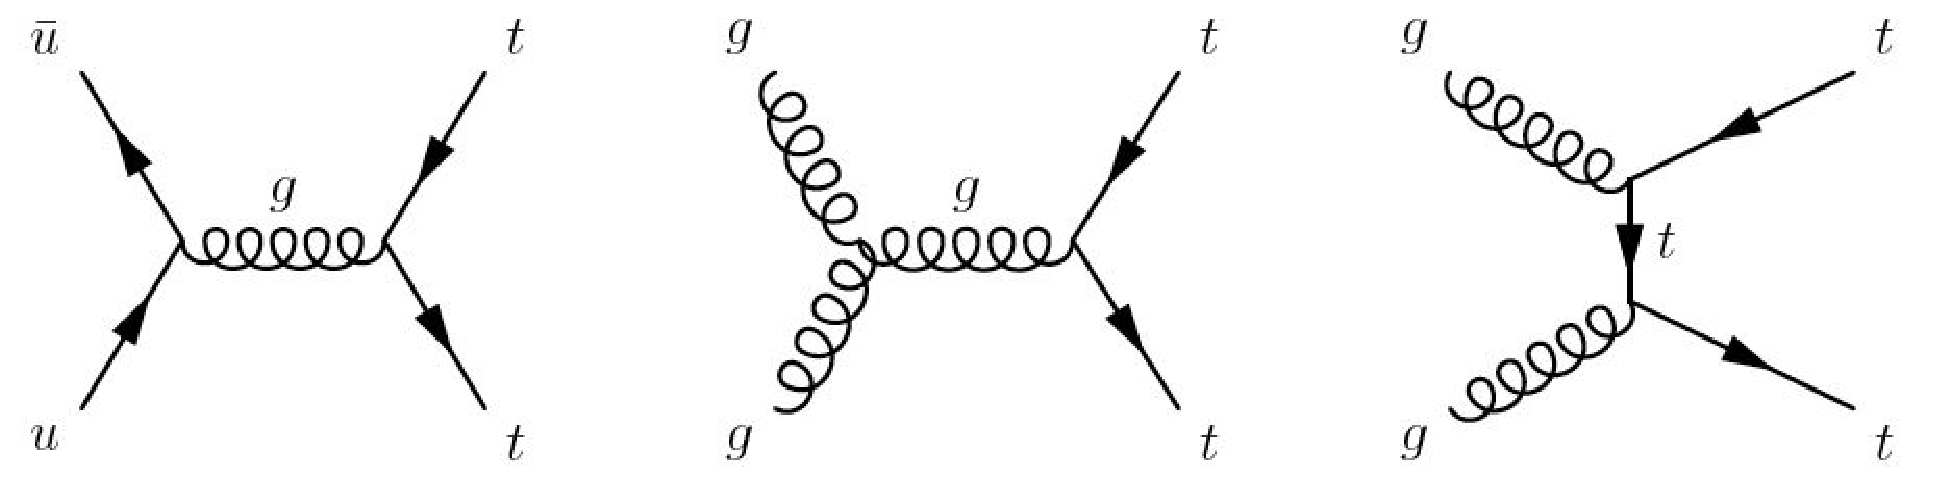
\includegraphics[width=0.9\textwidth]{eps/Theory/TTbar.eps}
\end{center}
\vspace{-0.1in}
\caption{Main leading order $t\bar{t}$ pair production Feynman diagrams~\cite{Jabeen:2006km}.}
\label{ttbar}
\end{figure}

\section{Electroweak Top Quark Production}
\label{electroweaktopquark}

Top quarks can also be produced via an electroweak interaction commonly called single top because only one top quark is produced in the event. At the Tevatron there are two dominant modes of single top production. The first is the $s$-channel process defined by a virtual time-like ($Q^{2}_{W} > 0$) $W$ boson formed from a $q\bar{q}'$ annihilation and decaying to a top and bottom quark. The second is the $t$-channel process defined by a virtual space-like ($Q^{2}_{W} < 0$) $W$ boson produced by a light and bottom quark exchange and producing a forward scattered light quark and a top quark. There is a third mode of production where the top quark is created in association with an on-shell ($Q^{2}_{W}=M^{2}_{W}$) $W$ boson; however, the cross section for this production mode is negligible at the Tevatron. Feynman diagrams for the $s$-channel and $t$-channel production modes are shown in Figs.~\ref{schannel} and~\ref{tchannel}.  The $s$-channel and $t$-channel cross sections have been calculated in~\cite{Smith:1996ij,PhysRevD.56.3114,Stelzer:1997ns,Harris:2002md,Sullivan:2004ie,Cao:2004ap,Cao:2005pq,Kidonakis:2006bu} with the cross sections used in the data analysis shown in Table~\ref{singletopcross}.

\begin{figure}[!h!tbp]
\begin{center}
\includegraphics[width=0.45\textwidth]{eps/Theory/schannel.eps}
\end{center}
\vspace{-0.1in}
\caption{The leading order Feynman diagram for the $s$-channel single top production mode~\cite{Jabeen:2006km}.}
\label{schannel}
\end{figure}

\begin{figure}[!h!tbp]
\begin{center}
\includegraphics[width=0.50\textwidth]{eps/Theory/tchannel.eps}
\end{center}
\vspace{-0.1in}
\caption{The leading order (left) and an important next-to-leading order (right) Feynman diagrams for the $t$-channel single top production mode~\cite{Jabeen:2006km}.}
\label{tchannel}
\end{figure}

As stated earlier in this chapter, the top quark prefers to decay to a $W$ boson and a $b$~quark. The common decay mode to detect single top events is when the $W$ boson either decays to an electron or muon and an associated neutrino\footnote{The $W\rightarrow \tau \nu_{\tau}$ and $W\rightarrow q\bar{q}^{'}$ channels are not considered in this thesis due to the large expected background rate.}. For the $s$-channel, the final state particles for the leading order process are (1) lepton, (1) neutrino, and (2) $b$ quarks. The $t$-channel final state is characterized by (1) lepton, (1) neutrino, (1) light quark, and at least one (1) $b$ quark. The $s$-channel and $t$-channel processes are sometimes referred to as $tb$ and $tqb$, respectively.

\vspace{0.2in}
\begin{table}[!h!tbp]
\begin{center}
\caption{Total cross sections for single top quark
production at $\sqrt{s} = 1.96$~TeV with $m_t=175$~GeV.}
\label{singletopcross}
\begin{minipage}{2.2 in}
\begin{tabular}{lc}
Process & Cross Section [pb] \\
\hline
$s$-channel ($tb$)	&	$0.88 \pm 0.11$		\\
$t$-channel ($tqb$)	&	$1.98 \pm 0.25$		\\
$s+t$			&	$2.86 \pm 0.27$		\\
\end{tabular}
\vspace{-0.1 in}
\end{minipage}
\end{center}
\end{table}



\subsection{Motivation for Single Top}
\label{motivation}

Measuring the single top quark production cross section ($\sigma$) and the angular differential cross section ($\frac{d\sigma}{d\Omega}$) is interesting as a test of the Standard Model as well as a probe for new physics beyond the Standard Model. Perhaps the most interesting product of a single top quark cross section measurement is a direct determination of the CKM matrix element $|V_{tb}|$ since the cross section is proportional to the square of this quantity ($\sigma\propto|V_{tb}|^{2}$).
If one assumes a unitary 3x3 CKM matrix then by measuring $|V_{ub}|$ and $|V_{cb}|$, $|V_{tb}|$ is required to be within the following range:
\begin{equation}
0.9991 < |V_{tb}| < 0.9994
\label{vtb}
\end{equation}

By relaxing the assumption on a unitary 3x3 CKM matrix~\cite{PhysRevD.63.014018}, $|V_{tb}|$ is allowed in the following range:
\begin{equation}
0.06 < |V_{tb}| < 0.9994
\end{equation}

A measurement of $|V_{tb}|$ that differed significantly from the range shown in Eq.~\ref{vtb} would be clear evidence for physics beyond the Standard Model such as a fourth generation of quarks.

Another interesting test of the Standard Model that can be made as a result of measuring single top is to probe the structure of the $Wtb$ vertex. In the Standard Model all single top quarks are produced via the left-handed electroweak interaction. If one were to boost into the top quark rest frame and know the four momenta of the decay products, then the angular decay distribution for the charged lepton from the $W$ boson decay would follow the distribution shown in Eq.~\ref{decay} where the angle $\theta_{l}$ is calculated with respect the top quark spin vector.

\begin{equation}
\frac{1}{\sigma}\frac{d\sigma}{d(\cos(\theta_{l})} = \frac{1}{2}\left[ 1 + \cos(\theta_{l}) \right]
\label{decay}
\end{equation}

In practice, boosting into the correct top quark frame does not always result in 100$\%$ left handed polarized ($\hat{s} \bullet \hat{p}=-1$) top quarks~\cite{Mahlon:1998uv}. For the $s$-channel process there an ambiguity resulting from the possibility of the up-type quark originating from the proton and the down-type quark origination from anti-proton and the reverse case. By boosting into the top quark frame and choosing the spin of the top quark along the direction of the anti-proton, one can expect to measure 98$\%$ polarization of top quarks. For the $t$-channel, the addition of higher order diagrams reduces the fraction of polarized top quarks. By boosting into the top frame and choosing the spin of the top quark along the direction of the forward down-type quark as seen in Fig.~\ref{tchannel}, one expects to measure 96$\%$ of top quarks to be polarized. By measuring the degree to which top quarks are polarized one can test the left-handed structure of the $Wtb$ vertex.

Finally, the $s$ and $t$-channel cross sections are sensitive to new particles predicted by theories beyond the Standard Model~\cite{PhysRevD.63.014018}. The Standard Model $s$-channel amplitude will interfere with any other diagram that includes a charged vector boson as the interaction mediator. One example of such a boson is the $W^{'}$ which results from an additional SU(2) group structure in the electroweak Lagrangian. The leading order Feynman diagrams for the $W^{'}$ boson production is shown in Fig.~\ref{schannelnew}.

\begin{figure}[!h!tbp]
\begin{center}
\includegraphics[width=0.45\textwidth]{eps/Theory/wprime.eps}
\end{center}
\vspace{-0.1in}
\caption{The leading order Feynman diagrams for the $s$-channel like process involving a $W^{'}$ boson~\cite{Jabeen:2006km}.}
\label{schannelnew}
\end{figure}

The Standard Model $t$-channel diagram will interfere primarily with new diagrams that involve flavor changing neutral currents (FCNC) including the top quark, which are predicted by models such as supersymmetry and technicolor~\cite{PhysRevD.63.014018}. A leading order Feynman diagram for this process is shown in Fig.~\ref{tchannelnew}.

\begin{figure}[!h!tbp]
\begin{center}
\includegraphics[width=0.2\textwidth]{eps/Theory/FCNC.eps}
\end{center}
\vspace{-0.1in}
\caption{A leading order Feynman diagram for a $t$-channel-like process produced through FCNC~\cite{Jabeen:2006km}.}
\label{tchannelnew}
\end{figure}

Thus, by measuring each production cross section to high accuracy, one can test the validity of new physics models.



\subsection{Signal Event Generation}
\label{singletopgeneration}

An important part of a physics analysis is to have a determination of the kinematic distributions of signal events along with a cross section estimate to provide a normalization for the number of events to expect from the $\ppbar$~collisions. Both of these tasks can be accomplished by Monte Carlo generators. Monte Carlo generators use a set of random numbers to sample the N-dimensional phase space defined by the number of initial and final state particles in the event. The trial event is given a weight determined by the differential cross section, shown in Eq.~\ref{diffcross}, and is selected as a signal event if the weight is greater than a new random number sampled from the properly normalized differential cross section distribution. This method allows for more events to be selected from a region in phase space where the differential cross section is large and few events are selected from regions of low differential cross section. The final step of the Monte Carlo simulation is to hadronize\footnote{Hadronization is the process of forming bound states (hadrons) between two or three quarks. A bound state of two quarks is called a meson and a three quark bound state is called a baryon.} and shower\footnote{A shower, or parton shower, is the result of multiple gluon emission from final state particles.} the final state partons and allow for additional energy in the event resulting from the breakup of the two protons in the collision. This final step is performed using the Pythia~\cite{Sjostrand:2001yu} Monte Carlo generator.

\begin{equation}
\label{diffcross}
\pderiv{\sigma(\vec{y})}{\vec{y}} = \sum_{i,j} f_{i}(Q^{2},x_{1})f_{j}(Q^{2},x_{2}) \times \pderiv{\sigma_{hs,ij}(\vec{y})}{\vec{y}}
\end{equation}

In Eq.~\ref{diffcross}, $\pderiv{\sigma_{hs,ij}(\vec{y})}{\vec{y}}$ is the differential cross section for the parton-parton\footnote{A parton is a constituent particle within the proton.} collision and $f_{i}(x_{1},Q^{2})$ and $f_{j}(x_{2},Q^{2})$ are the parton distribution functions (PDFs) that describe the number density of partons $i$ and $j$ inside the proton. The two parameters in these functions are the proton momentum fraction ($x=p_{\rm{parton}}/p_{\rm{proton}}$) and the energy scale (factorization scale) at which the two partons collide (Q). A plot of the parton density functions from the CTEQ~\cite{Pumplin:2002vw} collaboration is shown in Fig.~\ref{cteqpdfs} for two distinct momentum transfers. 

\begin{figure}[!h!tbp]
\begin{center}
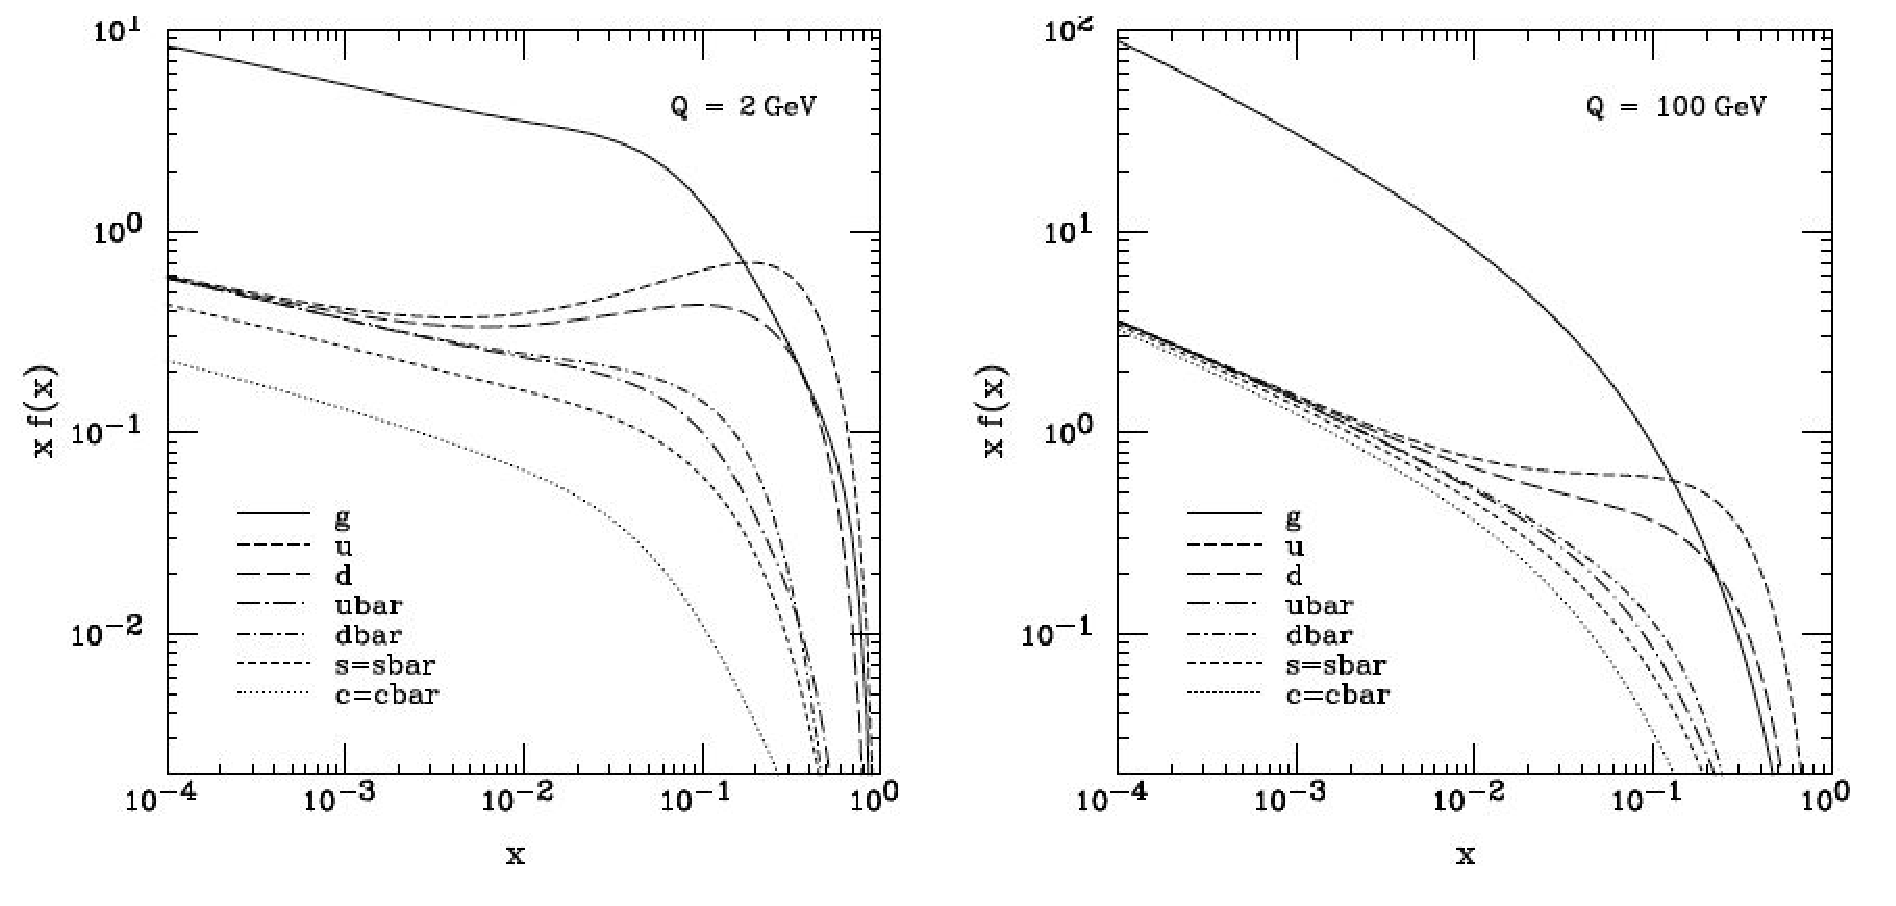
\includegraphics[width=0.90\textwidth]{eps/Theory/CTEQ_pdfs.eps}
\end{center}
\vspace{-0.1in}
\caption{CTEQ 6M parton distribution functions for the gluon and all quark flavors for a small momentum transfer (left) and large momentum transfer (right). The $x$-axis is the proton momentum fraction of the parton and the $y$-axis is the parton density~\cite{Pumplin:2002vw}.}
\label{cteqpdfs}
\end{figure}


Single top signal events are generated using the CompHEP based SingleTop~\cite{Boos:SingleTop} Monte Carlo generator. The following two sections describe the generation of $s$-channel and $t$-channel production. All events were generated using CTEQ6L1 PDFs. The $s$-channel events were generated with $Q^{2}=m_{t}^{2}$ and $t$-channel events were generated with $Q^{2}=(m_{t}/2)^{2}$.

\subsubsection{$s$-channel Generation Using CompHEP}
\label{schannelgen}

It has been shown in~\cite{Sullivan:2004ie} that $s$-channel kinematic distributions between leading order (LO) and next-to-leading order (NLO) in $\alpha_{s}$ are the same up to an overall normalization. The ratio of NLO to LO events, called a k-factor, is $1.3$~for the $s$-channel production mode. Fig.~\ref{schannelevents} shows the transverse momentum ($p_{T}$) and pseudorapidity\footnote{The pseudorapidity is related to the polar angle $\theta$. More discussion of this variable is given in Chaper~\ref{experiment}.}($\eta$) distributions for $s$-channel events generated by SingleTop.


\begin{figure}[!h!tbp]
\begin{center}
\includegraphics[width=0.49\textwidth]{eps/Theory/Hist_tb_Pt.eps}
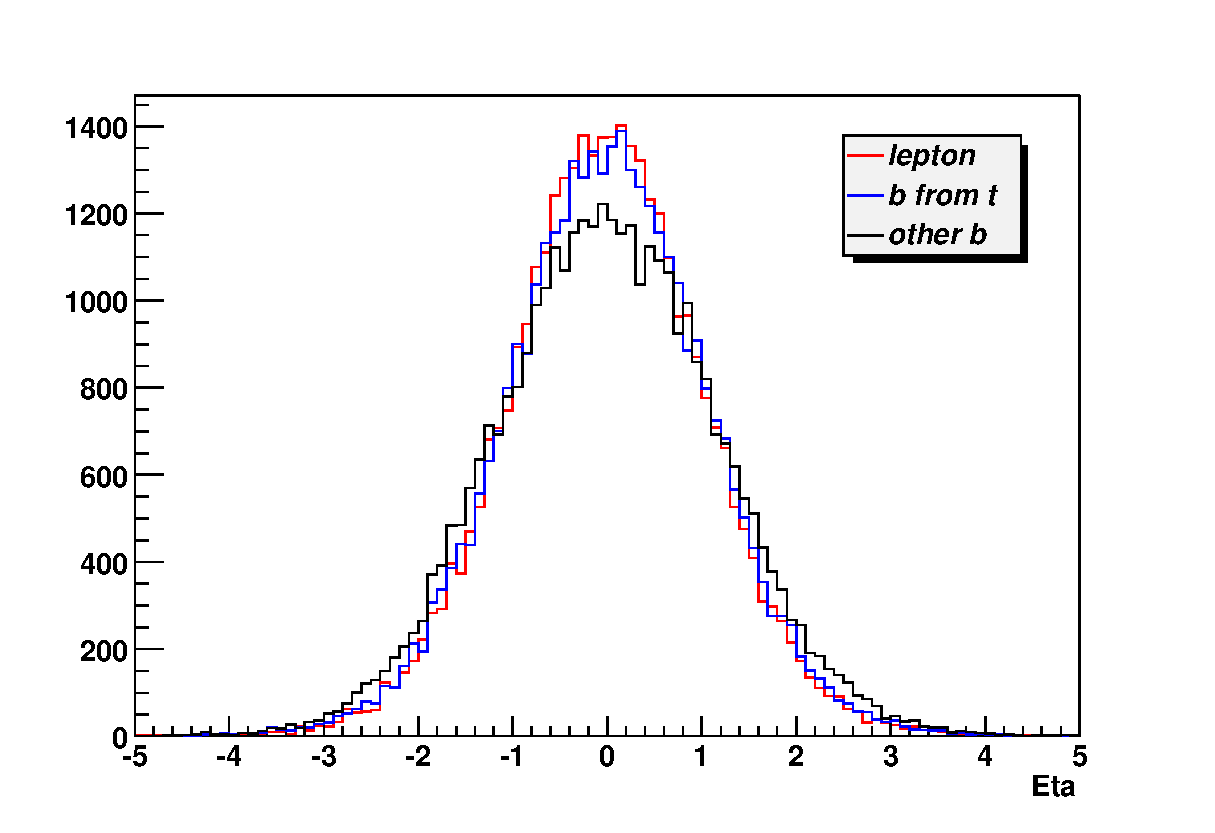
\includegraphics[width=0.49\textwidth]{eps/Theory/Hist_tb_Eta.eps}
\end{center}
\vspace{-0.1in}
\caption{$p_{T}$ (left) and $\eta$ (right) distributions of final state particles in $s$-channel events~\cite{Jabeen:2006km}.}
\label{schannelevents}
\end{figure}


\subsubsection{$t$-channel Generation Using CompHEP and Pythia}
\label{tchannelgen}

Generating $t$-channel Monte Carlo events is slightly more difficult than $s$-channel events because the effective cross section of higher order Feynman diagrams ($qg\rightarrow q^{'}tb$), shown in Fig.~\ref{tchannel}, is of the same order as the leading order diagram ($qb\rightarrow tq^{'}$). A proper treatment of the combination is required to avoid double counting regions of phase space where the two matrix elements overlap. The SingleTop generator avoids double counting by defining two distinct regions of phase space where the different processes are the dominant contribution to the total $t$-channel cross section. The first region of phase space is defined by $p_{T}(b)<10$~GeV. In this region the final state $b$~quark is produced by Pythia through initial state radiation (ISR). The second phase space region is defined by $p_{T}(b)>10$~GeV. In this region the $b$~quark is produced by the next-to-leading order Feynman diagram shown in Fig~\ref{tchannel}. To ensure a smooth transition from low to high $b$~quark $p_{T}$, the weight for the low $p_{T}$ region is multiplied by a k-factor to make the leading order Pythia generated $b$~quark $p_{T}$~match the next-to-leading order $b$~quark $p_{T}$ distribution. The k-factor used at the Tevatron is 1.21 and the effective NLO cross section used in the SingleTop generator is shown in Eq.~\ref{tchannelcross}.

\begin{equation}
\label{tchannelcross}
\sigma_{\rm{NLO}} = K\sigma_{\rm{Pythia}}|_{P_{T}(b)<10} + \sigma_{\rm{CompHEP-SingleTop}}|_{P_{T}(b)>10}
\end{equation}

The result of the $b$~quark $p_{T}$ splicing is an almost exact reproduction of many NLO differential distributions. Fig.~\ref{tchannelevents} shows $p_{T}$ and $\eta$ distributions for $t$-channel events generated by SingleTop.

\begin{figure}[!h!tbp]
\begin{center}
\includegraphics[width=0.49\textwidth]{eps/Theory/Hist_tqb_Pt.eps}
\includegraphics[width=0.49\textwidth]{eps/Theory/Hist_tqb_Eta.eps}
\end{center}
\vspace{-0.1in}
\caption{$p_{T}$ (left) and $\eta$ (right) distributions of final state particles in $s$-channel events~\cite{Jabeen:2006km}.}
\label{tchannelevents}
\end{figure}


